\section{Introduction}

We introduce some auxiliary concepts and formulate general assumptions:

\begin{itemize}
\item
A \emph{bit stream} is an array containing elements of type \verb"uint8_t".

A bit stream of length $n$ contains $8n$ bits.

\item
A bit stream is \emph{valid} if the array is valid.

\item 
A bit stream can be indexed both by its array indices
and its \emph{bit indices}.

Figure~\ref{fig:bitstream-indices} shows the difference between 
array indices and bit indices in a bit stream.
The two bit indices, 0~and~14,
mark bit positions in the first and second array element, respectively.

\begin{figure}[hbt]
\begin{center}

\includegraphics[width=0.40\textwidth]{figures/array_as_stream.pdf}
\caption{\label{fig:bitstream-indices} Array indices and bit indices in a bit stream}
\end{center}
\end{figure}


\item
A \emph{bit sequence} is a consecutive sequence of bits within a bit stream
as represented in Figure~\ref{fig:bitsequence}.
\begin{figure}[hbt]
\begin{center}
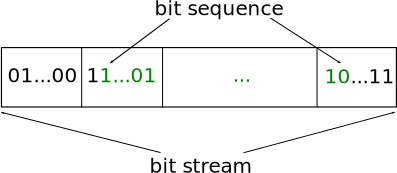
\includegraphics[width=0.40\textwidth]{figures/bit_sequence.pdf}
\caption{\label{fig:bitsequence} A bit sequence within a bit stream}
\end{center}
\end{figure}

A bit sequence is given by the position of its first bit (a bit index in the bit stream)
and its \emph{length}, that is, the number of bits it contains.

\item A bit sequence of length $l$ that starts at bit index $p$ is \emph{valid}
     with respect to a bit stream of length $n$ if the following conditions are
     satisfied
     \begin{align*}
         0 &\leq p \leq 8n \\
         0 &\leq p + l \leq 8n
     \end{align*}

\item 
We assume that the C-types \texttt{unsigned int} and \texttt{int}
have a width of~32~bits.

\end{itemize}


